%!TEX root = ../SciVis.tex
Besides the height plot we also implemented stream tubes, which are also drawn in three-dimensions. Stream tubes trace particles through a vector field as cylindrical tube. In contrast, to  height plots, stream tubes visualize a three-dimensional dataset. 

Therefore we need to construct a 3D dataset out of our 2D dataset by using time as the third axis. Basically, we store the last $n$ timeslices of our 2D dataset to create a data cube. 

We designed this data cube as a circular buffer. We decided to store all data that becomes available in every simulation step (i.e. rho,vx,vy,fx,fy). This gives us a greater flexibility since we are able to calculate all kinds of conversion on the fly (e.g. $|v|$).  
Deque and vector have been used to define the circular buffer as \verb| deque<vector<vector<fftw_floats> > > >|.  A deque  allows to easily push and pop data at both ends, which makes the implementation easier. 
We used the available STL data structures because they are reliable and effiecent.
The RHO value of a sample point $sp$  at timestep $t$ can be accessed via  \verb|buffer[t][RHO][sp]|. The data structure has been wrapped in a class to allow uniform access and provide general purpose methods. 


If we visualize this dataset by using a simple hedgehog glyph technique as described previously, we can see the different time slices (cf. Figure~\ref{fig:datacube_bottom}) or how the colors is propagated to the later time slices  Figure~\ref{fig:datacube_front}). However, due to occlusion it is difficult to look inside the dataset  and see how individual vectors change over time. While this visualization focusses on displaying all data, stream tubes limit the amount of presented data. Also stream tubes ha advantages (less occlusion) and disadvantages (incomplete picture on the data).

 \begin{figure}[htbp]
 \centering
 \begin{minipage}[t]{0.48\textwidth}
 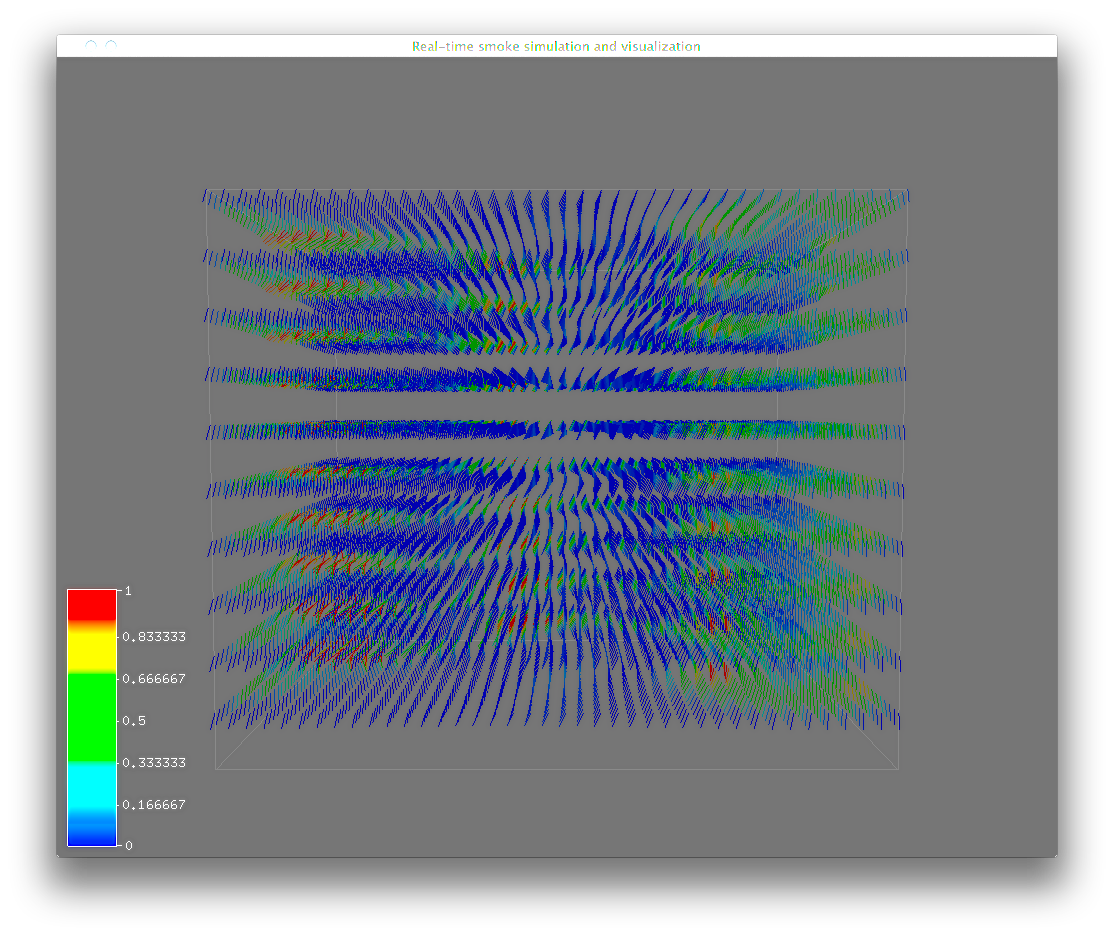
\includegraphics[height=3in]{figures/streamtubes/30datacube_bottom.png}
 \caption{Hedgehog visualization of the time-dependent velocity vector field. The individual time-slices are clearly visible if viewed from below.}
 \label{fig:datacube_bottom}
 \end{minipage}\hspace{.04\textwidth}%
 \begin{minipage}[t]{0.48\textwidth}
 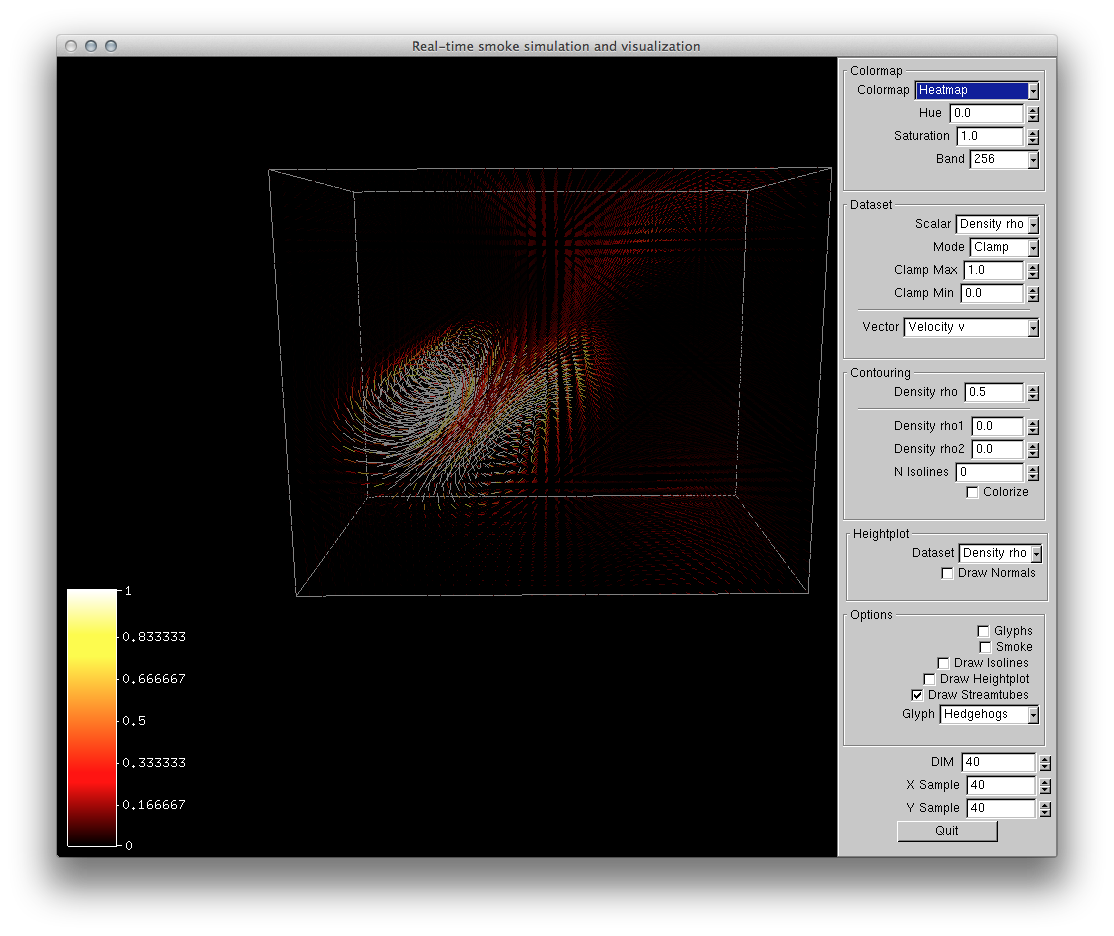
\includegraphics[height=3in]{figures/streamtubes/31datacube_front.png}
 \caption{Frontal view of the the time-dependent velocity vector field. Occlusion is a problem as the individual vectors/time slices cannot be easily perceived.}
 \label{fig:datacube_front}
 \end{minipage}
 \end{figure}
 
 
 One problem of stream tubes is the selection of seed points (start point of the trace). In  this case, the user has the possibility to specify the seed points on his own either by selecting the value on the x,y,z slider or by clicking onto the screen. The user can specify as many seed points as he wants. 
 
The stream tube algorithm is a straightforward extension of the stream line algorithm. Instead of operating on a cell with four sample points, the algorithm operates on cubes with eight sample points. In order to find the direction for the next integration step, the vector is obtained by trilinearly  interpolating x,y,z. However, z is constant since it represent the time.
The resulting point will be pushed on a vector of points, which will be used to draw the actual steam tube along the calculated values. 
Similar to stream lines the quality and length of the traces can be influenced by increasing or decreasing the integration step and defining  stop criteria.


\begin{figure}[htbp]
\centering
\begin{minipage}[t]{0.48\textwidth}
        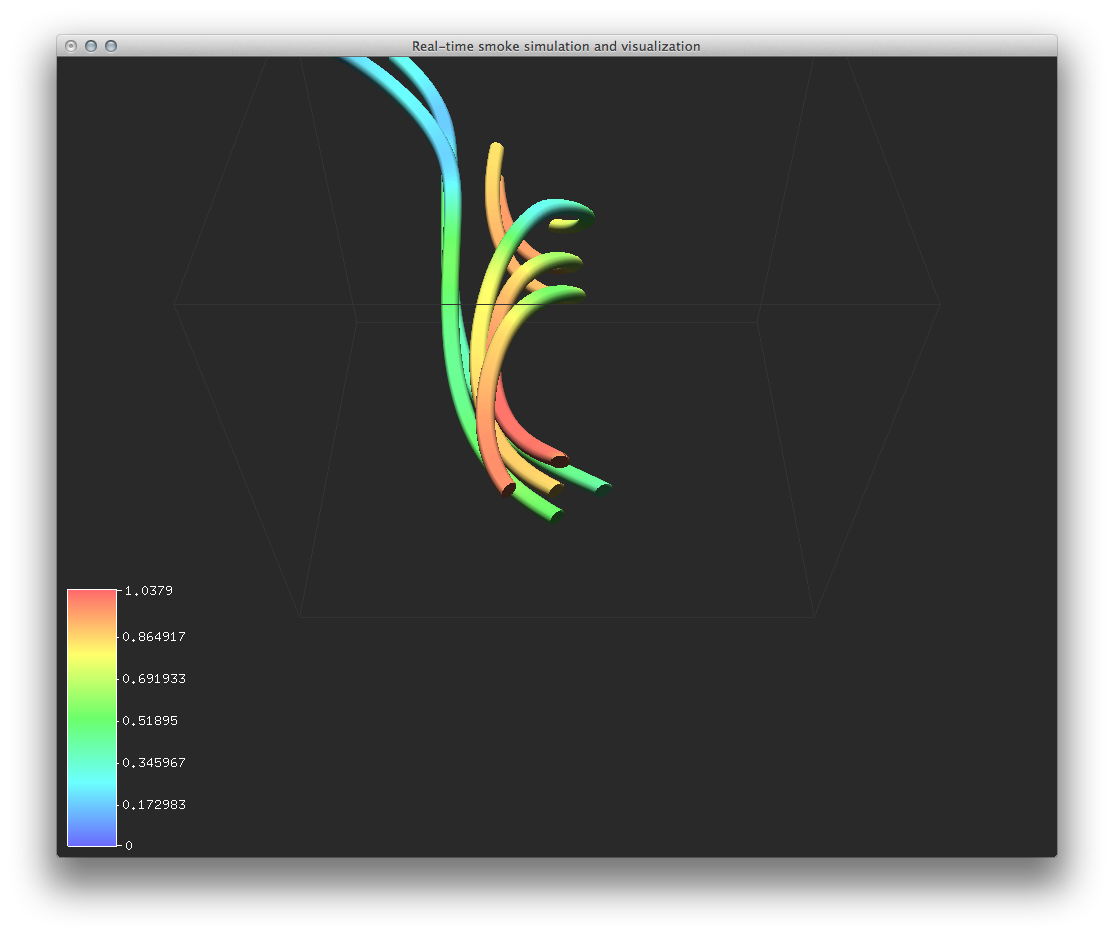
\includegraphics[height=3in]{figures/streamtubes/10tubes.png}
\caption{Combination of streamtubes and colormapping. Both techniques show the velocity. The seedpoints are centered in middle of the dataset.}
\label{fig:}
\end{minipage}\hspace{.04\textwidth}%
\begin{minipage}[t]{0.48\textwidth}
    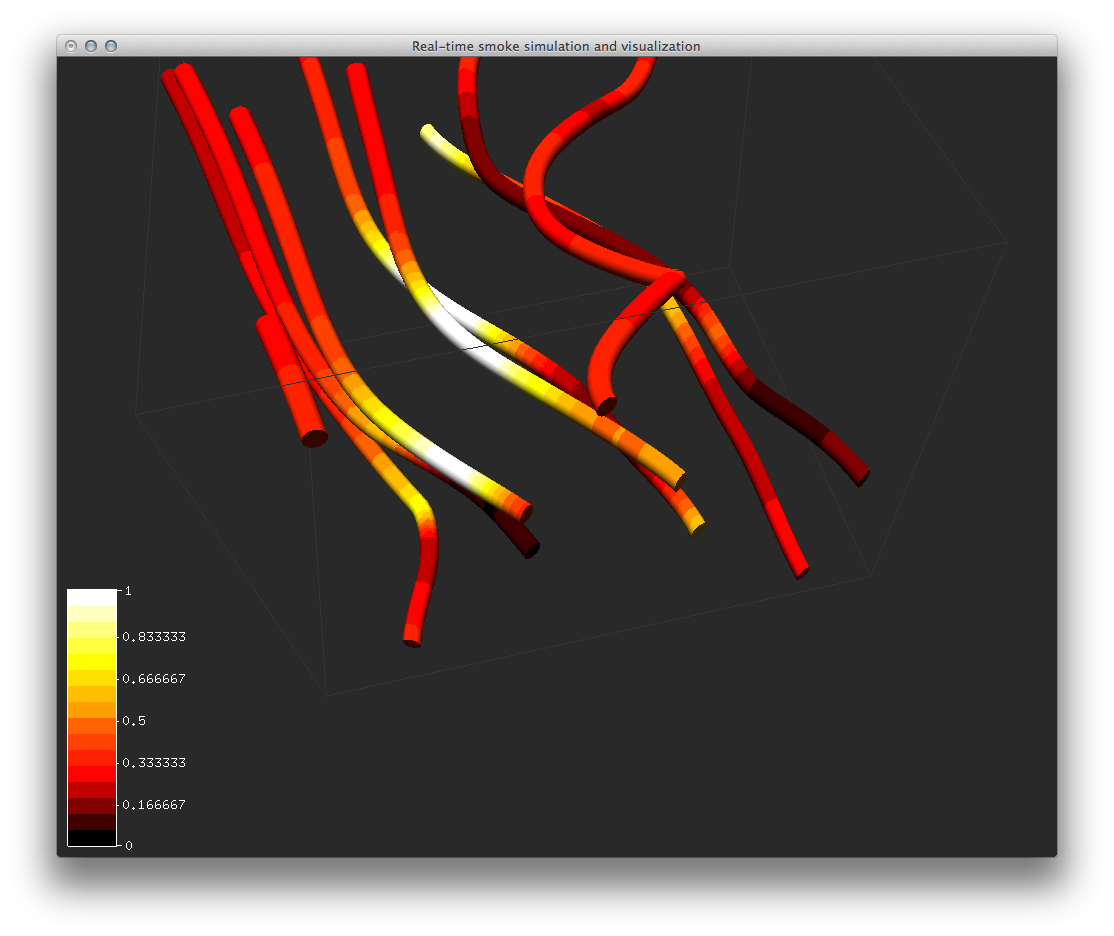
\includegraphics[height=3in]{figures/streamtubes/21banding_velodensity.png}
    \caption{Visualization of the velocity as streamtubes and density as heat colormap with a reduced number of colors. The banding effect makes the integration steps visible.}
    \label{fig:}
\end{minipage}
\end{figure}

In order to construct the tubes geometry out of the calculated stream points, we use a 3D reference frame that contains a cross section. This reference frame will be placed along the streamline to create a closed tube. We used a circular cross-section that allows to define the number of segments (cf. Listing~\ref{lst:reffr} ad Figure~\ref{fig:trangTubes}). The cross-section also calculates the  (surface) normals (cf. Figure~\ref{fig:shadedtubes}) and allows to adjust the thickness of the tube based on a scalar value (cf. \ref{fig:thicktubes}). 
  
\begin{lstlisting}[language=C,caption={Cross-section in 3D reference frame},label=lst:reffr]
glBegin(GL_QUAD_STRIP);
  for (int i = 0; i <= 360; i = i + (360 / n)) {
    float theta = i * (M_PI / 180);
    float theta2 = (i + 1)*(M_PI / 180);
    
    float normal[3] = {};
    float vz[3] = {
        (cos(theta) * r) - (cos(theta) * rn),
        (sin(theta) * r)-(sin(theta) * rn),
         10 
    };
    float vx[3] = {
        (cos(theta) * r) - (cos(theta2) * r),
        (sin(theta) * r)-(sin(theta2) * r),
        0
    };
    normalize3(vz);
    normalize3(vx);
    crossproduct(vz, vx, normal);

    setColor(points[sp][3], TEXTURE);
    glNormal3f(normal[0], normal[1], normal[2]);
    glVertex3f(cos(theta) * r, sin(theta) * r, 0);

    setColor(points[sp + 1][3], TEXTURE);
    glNormal3f(normal[0], normal[1], normal[2]);
    glVertex3f(cos(theta) * rn, sin(theta) * rn, 15);

    setColor(points[sp][3], TEXTURE);
    glNormal3f(normal[0], normal[1], normal[2]);
    glVertex3f(cos(theta2) * r, sin(theta2) * r, 0);

    setColor(points[sp + 1][3], TEXTURE);
    glNormal3f(normal[0], normal[1], normal[2]);
    glVertex3f(cos(theta2) * rn, sin(theta2) * rn, 15);
  }
glEnd();
\end{lstlisting}  
  
 In order to sweep the cross-section along the stream tube we need to find a transformation matrix that performs the correct translation and rotation of the reference frame. By using the cross product and the previous stream point we can obtain three vectors. One vector is tangent to the direction of the next segment and the other one is perpendicular to the tangent vector and shows the local up-direction. The third vector shows the local x direction.  The vectors are illustrated in Figure~\ref{fig:orientationVec}.
 
Having this information, the transformation matrix is constructed as shown in Listing~\ref{lst:translationMatrix}. The vector \verb|points[sp][]| is a simple spatial translation and puts the reference frame to the correct location.

 \begin{lstlisting}[language=C, caption={Rotation and translation matrix to move cross-section along the streamtube.},label={lst:translationMatrix}]
 GLfloat R[16] = {
     local[0]     , local[1]     , local[2]     , 0,
     up[0]        , up[1]        , up[2]        , 0,
     target[0]    , target[1]    , target[2]    , 0,
     points[sp][0], points[sp][1], points[sp][2], 1
 };
 glMultMatrixf(R);
 \end{lstlisting}
 
The stream tube technique is also able to visualize a vector and scalar dataset at the same time by coloring the tube using a color map as described in the previous sections about color mapping and height plots.

\begin{figure}[htbp]
\centering
\begin{minipage}[t]{0.48\textwidth}
        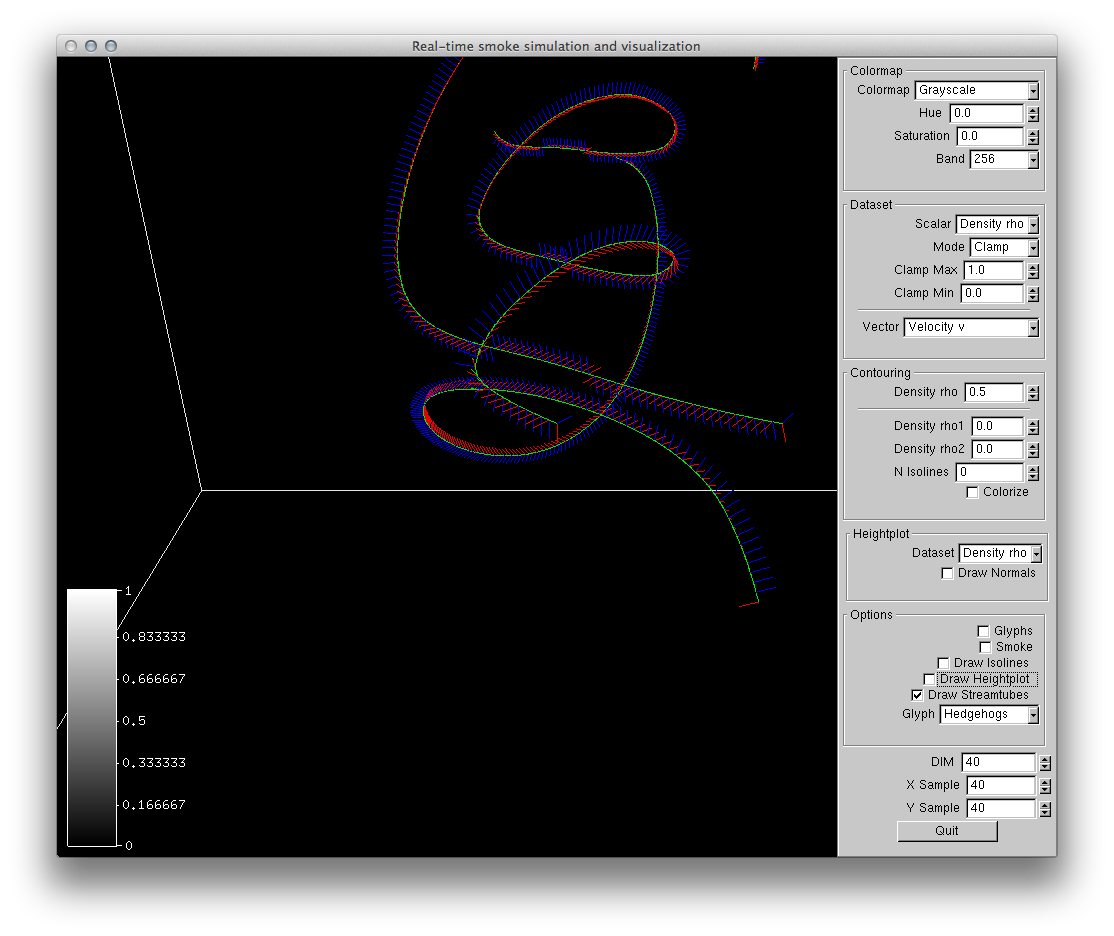
\includegraphics[height=3in]{figures/streamtubes/uvp.png}
\caption{Scaled orientation vectors. The green vector is tangent to the streamline, while the red and blue are perpendicular to the streamline.}
\label{fig:orientationVec}
\end{minipage}\hspace{.04\textwidth}%
\begin{minipage}[t]{0.48\textwidth}
               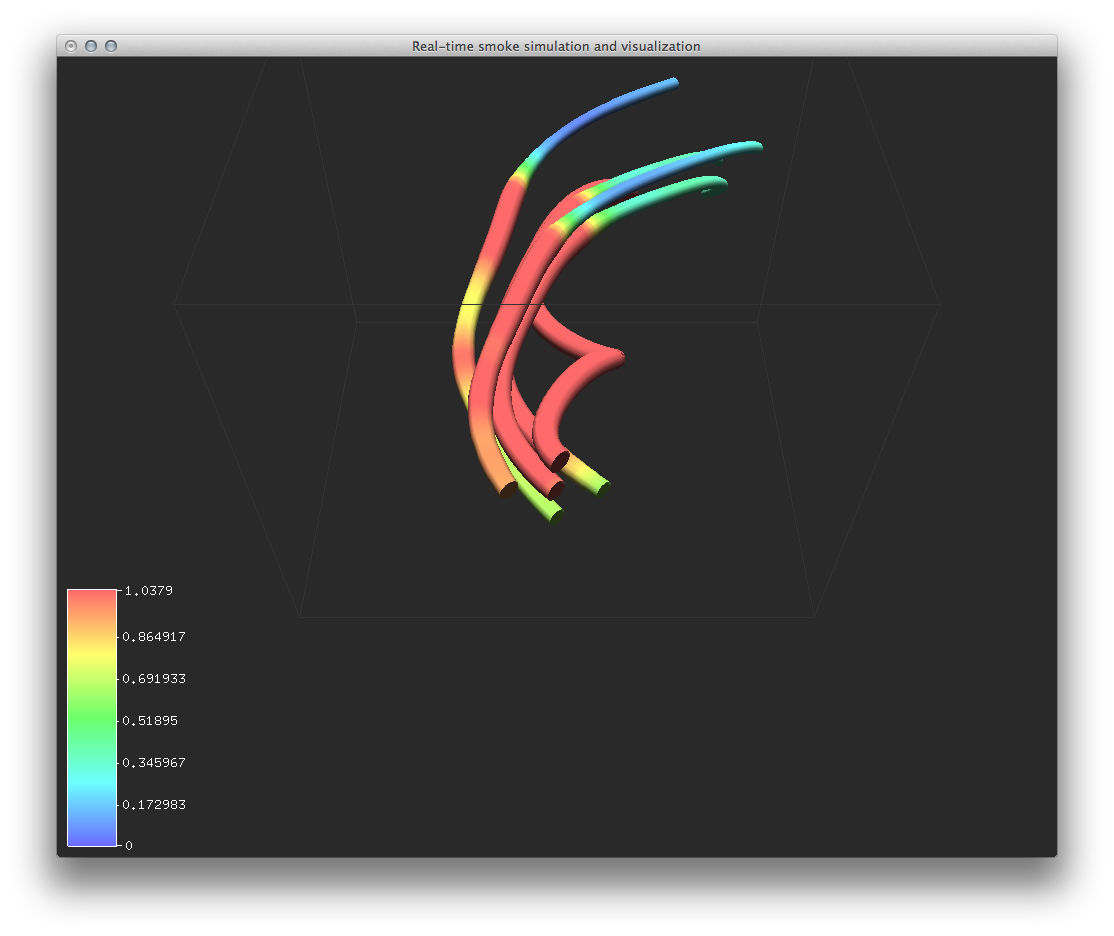
\includegraphics[height=3in]{figures/streamtubes/11thickTubes.png} 
    \caption{The diameter of the tube is linearly scaled based on a scalar value.}
    \label{fig:thicktubes}
\end{minipage}
\end{figure}



\begin{figure}[htbp]
\centering
\begin{minipage}[t]{0.48\textwidth}
        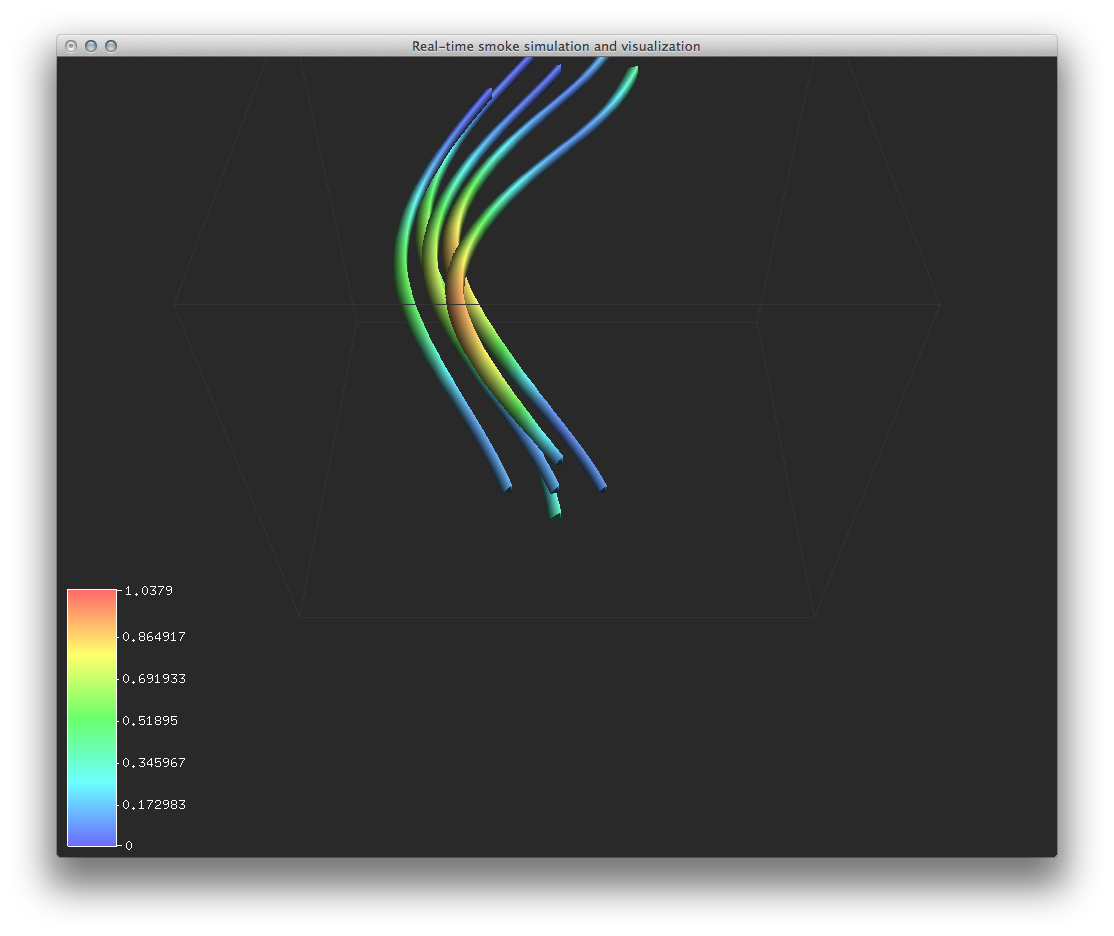
\includegraphics[height=3in]{figures/streamtubes/40threeSegments.png}
\caption{Triangular Tube geometry. The number of segments of the cross-sections can be adjusted dynamically.}
\label{fig:trangTubes}
\end{minipage}\hspace{.04\textwidth}%
\begin{minipage}[t]{0.48\textwidth}
        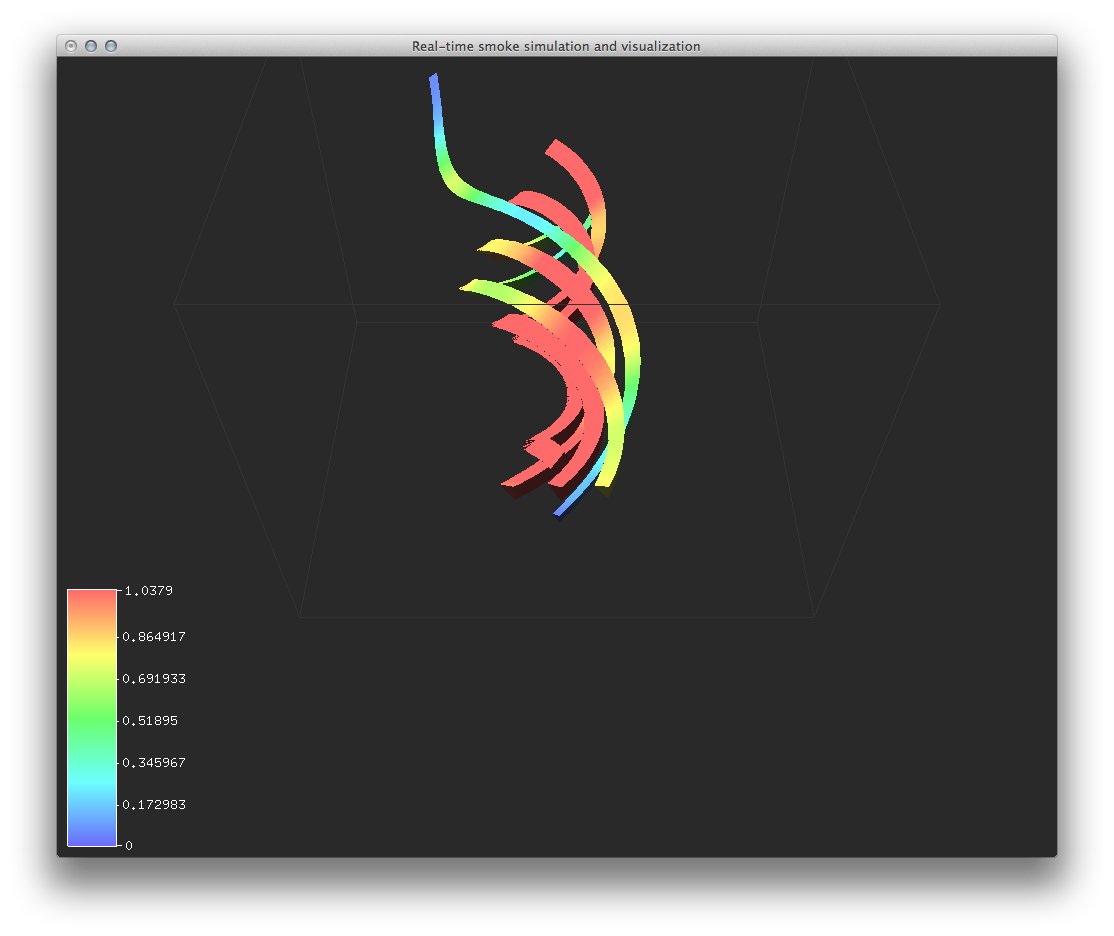
\includegraphics[height=3in]{figures/streamtubes/41flatshading.png}
    \caption{Flat shading accentuate the sharp-edges of the cross-section}
    \label{fig:shadedtubes}
\end{minipage}
\end{figure}

